\documentclass[a4paper, 14pt]{extarticle}
\usepackage[a4paper,top=2cm,bottom=2cm,left=3cm,right=1.5cm,margin=15mm, lmargin=30mm]{geometry}
\usepackage{lingmacros}
\usepackage[utf8]{inputenc}
\usepackage{tree-dvips}
\usepackage[utf8]{inputenc}
\usepackage[T2A]{fontenc}
\usepackage[english,russian]{babel}
\usepackage[autostyle]{csquotes}
\usepackage{amssymb}
\usepackage{amsfonts}
\usepackage{amsmath}
\usepackage{color}
\usepackage{graphicx}


\usepackage{tempora} %Times New Roman alike                                     
\usepackage{newtxmath} %Times New Roman in math




\begin{document}

1. Постановка задачи \\


Задача коммивояжера является одной из самых известных задач комбинаторной оптимизации. Изначально у нас имеется полный взвешенный граф, который является математической моделью для некоторых городов и расстояний между ними, где вершина графа это город, а ребра графа - это путь, пролегающий между городами. Вес ребра это длина пути или же стоимость проезда. Задача: найти путь минимальной стоимости, то есть найти гамильтонов цикл минимального веса. Гамильтоновым циклом в графе называется цикл, в который каждая вершина графа включена ровно один раз. Данная задача относится к классу NP-трудных задач. По этой причине для этой задачи актуально исследование приближенных алгоритмов с целью получения приемлемого решения за более короткий промежуток времени. \\
Одним из алгоритмов, находящих некое решение за приемлемое количество операций, $O(n^{2})$, где $n$ - количество вершин, является жадный алгоритм с выбором ближайшей вершины. Суть алгоритма заключается в том, что на каждом шаге мы просматриваем все непосещенные вершины в которые можно попасть из текущей вершины, и выбираем ту, расстояние до которой минимально. Оценку времени работы алгоритма получить нетрудно: на каждом шаге мы просматриваем не более n вершин и выбираем одну из них. Всего у нас $n$ вершин, значит будет $n$ шагов. Получаем оценку $O(n^{2})$. В общем случае данный алгоритм может работать сколь угодно плохо относительно оптимального решения. На изображении ниже представлен пример на котором жадный алгоритм, запущенный из любой точки будет работать сколь угодно плохо в зависимости от веса ребра.
*здесь будет пример плохой работы алгоритма*
Однако, если мы наложим дополнительные условия на веса ребер или сам граф мы можем получить более точный результат. Например, если граф метрический, у нас появляются верхняя и нижняя оценки оптимальности работы жадного алгоритма. \newline

Для маршрута коммивояжера с $n$ вершинами справедлива теорема:

\textbf{Теорема 1. Веерхняя оценка оптимальности:}

\begin{equation}
	(\frac{Greedy}{Optimal}) \leqq \frac{1}{2}\lceil{\lg n}\rceil + \frac{1}{2}
\end{equation}

Где $Greedy$ - вес пути, найденного жадным алгоритмом, $Optimal$ - вес наиболее оптимального пути.

Доказательство:

\textbf{Лемма 1}: Допустим существует отображение вершины $p$ в число $l_p$ такое, что:\\
1) $d(p,q) \geq min(l_p, l_q) \: \forall \: p,q$\\
2) $l_p \leq \frac{1}{2}OPT\: \forall \: p $\\
Тогда 
\begin{equation}
\sum l_p \leq \frac{1}{2}(\lceil lg(n)\rceil+1)Optimal
\end{equation}

Доказательство.
Допустим Б.О.О., что N такое, что  ${i ]1<=i<= n }$  и $l_i \geq l_j$ если $i \leq j$
Докажем, что 

\begin{equation}\label{metriclowerbound}
	{Optimal} \geqq \sum_{i=k+1}^{min(2k,n)}\mathrm{l}_i
\end{equation}

для любого $k$ такого что $l \leq k \leq $n
Пусть H полный подграф, определенный на множестве узлов

\begin{equation}
	{\{i|1 \leq i \leq min(2k, n)\}}
\end{equation}

Пусть $T$ - это маршрут коммивояжера в $H$, который посещает вершины $H$ в том же порядке, что и эти узлы посещаются при оптимальном обходе исходного графа. Обозначим длину маршрута $T$ как LENGTH. По неравенству треугольника каждое ребро (b, c) графа T должно иметь длину меньше или равную длине пути от b до c, вычисленного в оптимальном пути коммивояжера. Так как ребра $T$ суммируются в LENGTH, а сумма ребер оптимального пути равна OPTIMAL мы заключаем что
\begin{equation}
	{Optimal} \geqq {LENGTH}
\end{equation}

По условию 1) Леммы для каждого $(i, j)$ в пути T  $d (i, j)> = min (\mathrm{l}_i, \mathrm{l}_j)$. Следовательно,

\begin{equation}\label{metric2.3}
	{LENGTH} \geqq \sum_{(i,j)\in T}^{}min(\mathrm{l}_i,\mathrm{l}_j ) = \sum_{i\in H}^{} \mathrm{\alpha}_i\mathrm{l}_i
\end{equation}

где $a_i$ - количество ребер $(i, j)$ в $T$, для которых $i > j$ (и, следовательно, $l_i=min(l_i, l_j)$).
Мы хотим получить нижнюю оценку правой части \ref{metric2.3}. Заметьте, что каждое $a_i$ не превосходит 2 (потому что $i$ это конечная точка только двух ребер в маршруте T) и что сумма $a_i$ равна количеству ребер в $T$. Поскольку $k$ составляет не менее половины количества ребер в $T$, мы заведомо получим нижнюю оценку правой части \ref{metric2.3}, если мы предположим, что $k$ наибольших $l_i$ имеют $a_i=0$, а остальные $min (2k, n) - k$ из $l_i$ имеют $a_i= 2$. По предположению, $k$ наибольших $\{ l_i|1 \leq i \leq k\}$, поэтому оценка нижней границы:


\begin{equation}
	\sum_{i \in H} a_i l_i \geq 2 \sum_{i=k+1}^{min(2k, n)} l_i
	\label{sum}
\end{equation}

Таким образом мы доказали неравенство \ref{metriclowerbound}

Теперь просуммируем неравенства \ref{metriclowerbound} для всех $k$ равных степени двойки меньшей $n$, то есть:
\begin{equation}
\sum_{j=0}^{[lg(n)]-1} OPT \geq \sum_{j=0}^{[lg(n)]-1} 2* \sum_{i=2^j+1}^{min(2^{j+1}, n)} l_i
\end{equation}

Это можно упростить до

\begin{equation}
\lceil lg(n) \rceil OPT \geq 2* \sum_{i=2}^{n} l_i
\end{equation}

По условию 2) Леммы
\begin{equation}
OPT \geq 2*l_1
\end{equation}
Два данных неравенства доказывают лемму

Доказательство Теоремы 1. Для каждой  вершины $p$ положим, что $l_p$ это длина ребра, выходящего из p и идущего в вершину, которая выбирается жадным алгоритмом. Мы хотим показать, что $l_p$ удовлетворяет условиям Леммы 1. Если вершина $p$ была выбрана жадным алгоритмом до вершины $q$, тогда вершина $q$ была кандидатом на ближайшую невыбранную вершину для вершины $p$. Это значит, что ребро $(p,q)$ не короче чем выбранное ребро, то есть
\begin{equation}
d(p,q) \geq l_p
\end{equation}
И наоборот, если вершина $q$ была выбрана до $p$, тогда
\begin{equation}
d(p,q) \geq l_q
\end{equation}
Так как одна из вершин была выбрана раньше другой, одно из двух последних неравенств должно выполняться, вследствие чего  условие 1) Леммы 1 выполняется. Для доказательства условия 2) достаточно доказать, что для любого ребра $(p,q)$
\begin{equation}
d(p,q) \leq \frac{1}{2}OPT
\end{equation}
Мы можем рассмотреть оптимальный маршрут как объединение двух частей маршрута, каждый из которых это путь между $p$ и $q$. Из неравенства треугольника получаем, что длина любого пути между $p$ и $q$ не может быть меньше, чем $d(p,q)$, что доказывает неравенство выше. Так как $l_p$ это длины всех пар, составляющих маршрут $T$
\begin{equation}
\sum l_p = GREEDY
\end{equation}
Данное равенство вместе с Леммой 1 доказывают неравенство из Теоремы 1.




\textbf{Теорема 2. Верхняя оценка оптимальности:}
\begin{equation}
	(\frac{Greedy}{Optimal}) > \frac{1}{3}{\lg (n+1)} + \frac{4}{9}
\end{equation}

Доказательство:  Для каждого $i \geq 1 $ построим неполный взвешенный граф F с тремя особыми вершинами: левая вершина, центральная вершина и правая вершина. Эти графы строятся рекурсивно как показано на рис.1 (TODO нарисовать и вставить) где левая вершина располагается слева, правая - справа и центральная посередине. Каждый граф F имеет путь P, соединяющий левую вершину и центральную, в который входят все вершины графа. Путь P также строится рекурсивно как на рис.1. 

\begin{center}
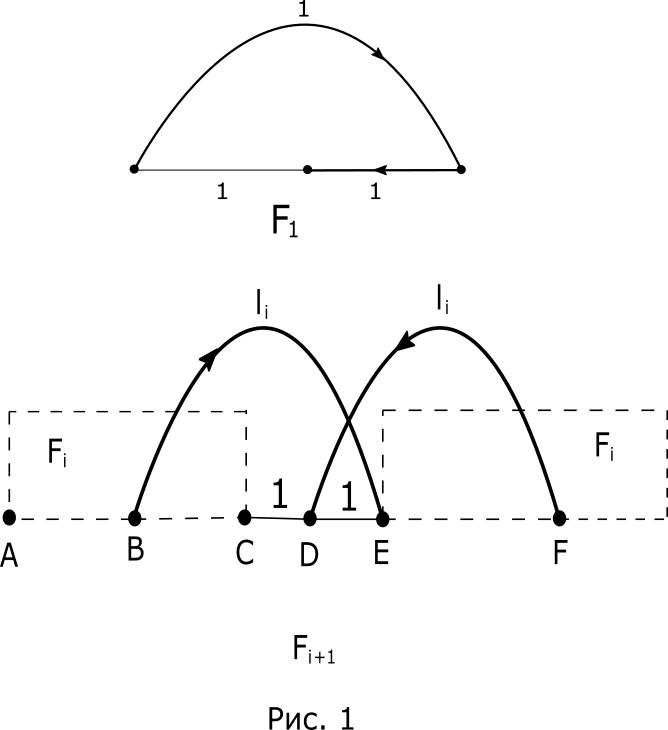
\includegraphics[width=200pt]{ris1.png}
\end{center}


Граф $F_1$ состоит из трех вершин, между каждыми двумя из которых проведено ребро веса 1. Путь P состоит из двух ребер: между левой и правой вершиной, между правой и центральной вершиной. Для построения графа $F_{i+1}$ возьмем две копии графа F, назовем одну копию левой, а другую правой. Добавим дополнительную вершину которая впоследствии станет центральной для $F_{i+1}$. На рис.1 эта вершина обозначена D. Она соединяется с правой вершиной левой копии (вершина C) и левой вершиной правой копии (вершина E) ребрами длины 1. Дополнительная вершина D также соединяется с центральной вершиной правой копии (вершина F) ребром веса $l_i$, который будет определен ниже. Наконец, центральная вершина левой копии (вершина B) соединяется с левой вершиной правой копии (вершина E) ребром веса $l_i$. Левая вершина $F_{i+1}$ определяется как левая вершина левой копии (вершина A), правая вершина $F_{i+1}$ определяется как правая вершина правой копии (вершина G). Путь $P_{i+1}$ состоит из двух копий пути $P_i$ и ребер (B,E), (F,D) длины  $l_i$. Длина $l_i$ данных ребер определяется по формуле
\begin{equation}\label{2.11}
l_i = \frac{1}{6}(4*2^i-(-1)^i+3)
\end{equation}
Пусть $L_i$ - длина пути $P_i$. Для длины $L_i$ есть рекуррентное соотношение:
\begin{equation}
L_{i+1} = 2*L_i+2*l_i
\end{equation}
Так как $P_{i+1}$ состоит из двух копий $P_i$ и двух ребер веса $l_i$ При условии что $L_1=2$, решение данного уравнения: 
\begin{equation}
L_i=\frac{1}{9}(6i*2^i+8*2^i+(-1)^i-9)
\end{equation}
Для каждого F мы определяем граф $G_i$, который получается из F путем соединения левой вершины и правой вершины графа ребром веса 1 и соединением центральной вершины с левой вершиной ребром веса $l_i-1$. Левая вершина графа F считается начальной вершиной графа $G_i$. На рисунке изображен граф $G_4$ Определим $\bar G_i$ как полный граф на вершинах $G_i$. Длина ребер в данном графе будет равна длине наименьшего пути в $G_i$ между двумя вершинами, которые соединяет ребро. Таким образом $\bar G_i$ будет удовлетворять неравенству треугольника.


\begin{center}
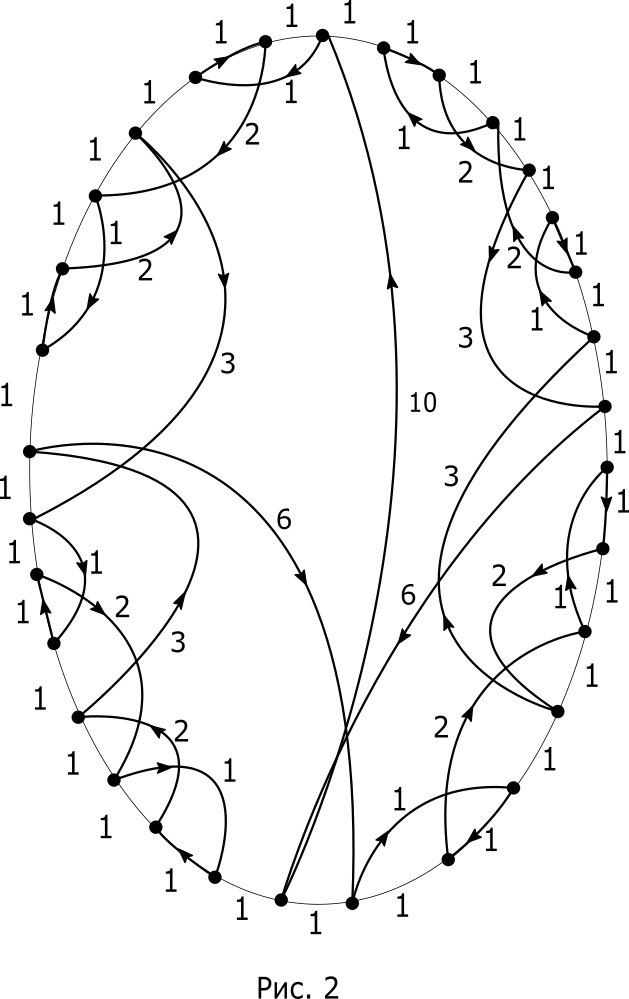
\includegraphics[width=200pt]{ris2.png}
\end{center}


Граф $\bar G_i$ имеет два важных свойства:\\
1) Ребра графа $G_i$ имеют в графе $\bar G_i$ такие же длины как и в $G_i$ \\
2) Если жадный алгоритм начинает свою работу с начальной вершины графа  $G_i$ то при подходящем выборе меджу несколькими возможными путями в алгоритме метод может найти путь $P_i$, который будет следовать за ребром длины $l_i-1$, проведенным из центральной вершины (последняя в пути $P_i$) в начальную вершину.

Мы вернемся к доказательству этих свойств после завершения доказательства основной теоремы.
Каждый граф $\bar G_i$ имеет оптимальный маршрут, состоящий из ребер единичного веса, с, соответственно весом пути равным n, где n - это количество вершин ($2^{i+1}-1$). Данный путь начинается в начальной вершине и далее посещаются все вершины слева направо, после чего происходит возврат в начальную вершину. Примером, удовлетворяющим теореме является граф $\bar G_{m-1}$ Соотношение для него:
\begin{equation}
\frac{GREEDY}{OPTIMAL} = (L_i+l_i-1)/n, \:  i=lg(n+1)-1
\end{equation}
Данное соотношение больше чем соотношение в теореме.
Остается доказать свойства 1) и 2).
Рассмотрим рис.1 TODO нумерация
Покажем что для каждого $F_{i+1}$
\begin{equation}\label{2.13}
\overline {AB}= \overline {BC}= \overline {EF}=\overline {FG}=l_i-1
\end{equation}
\begin{equation}\label{2.14}
\overline {AC}= \overline {EG}=l_{i+1}-2
\end{equation}
\begin{equation}\label{2.15}
\overline {BE}= \overline {DF}=l_i
\end{equation}
\begin{equation}\label{2.16}
\overline {AD}= \overline {DG}=l_{i+1}-1
\end{equation}
\begin{equation}\label{2.17}
\overline {AG}=l_{i+2}-2
\end{equation}
Запись $\overline {XY}$ означает длину кратчайшего пути между X и Y в графе $F_{i+1}$. Данные равенства тривиально доказываются для i=1. Далее будем вести доказательство по индукции. Предположим что равенства верны для $i \leq I-1$, например для $F_I$ На рис.3а изображены связанные вершины графа $F_{I+1}$ до объединения двух копий $F_I$ в $F_{I+1}$. Веса ребер графа равны кратчайшему пути между ними в $F_I$. Эти веса определены в предположении индукции. Например, ребро (A,B) на рис.3а соединяет левую и центральную вершины $F_I$ и, как следует из \ref{2.16}, длина кратчайшего пути между этими вершинами равна $l_i-1$. На рис.3б TODO мы можем увидеть фигуры с рис.3а TODO с ребрами, которые были добавлены при построении $F_{I+1}$. Так как каждый вес ребра между двумя вершинами на рис.3а равен кратчайшему пути между этими вершинами, то применяя формулу \ref{2.11} для $l_I$ ко всем возможным путям в $F_{i+1}$ мы можем найти, что вес каждого ребра на рис.3б  действительно является длиной кратчайшего пути между двумя вершинами, которые соединяет ребро. Это доказывает равенства \ref{2.13}-\ref{2.15} для $F_{I+1}$. Равенства \ref{2.16}, \ref{2.17} доказываются аналогичными рассуждениями для всех путей на TODO рис.3б. Путем длины $l_{i+1}-2$ из A в G является путь ABEG.





Объектом исследований данной работы являются оценки оптимальности решения задачи, найденного жадным алгоритмом при случае когда веса ребер являются случайными величинами и распределены по некоторому закону распределения. \\ \\
\textbf{2. Некоторые определения и вспомогательные теоремы} \\ 

\textbf{2.1 Определения}\\

Алгоритм $\mathcal{A}$ будем называть ассимптотически оптимальным если существуют такие $\epsilon_n \rightarrow 0, \delta_n \rightarrow 0$ при $n \rightarrow \infty$ что применение алгоритма $\mathcal{A}$ дает значение  $\mathcal{Z_A}$, удовлетворяющее неравенству
 
\begin{equation}\label{1}
P\{\mathcal{Z_A} \leq (1+\epsilon_n)\mathcal{Z}\}\geq 1-\delta_n
\end{equation}

где $\mathcal{Z_A}$ - решение, найденное алгоритмом, $\mathcal{Z}$ - минмальное решение.
Это определение при $\epsilon_n \equiv 0$ совпадает с понятием алгоритма, который почти всегда приводит к точному решению. \\

\textbf{2.2 Неравенство Чебышева} \\

Пусть случайная величина X: $\Omega\rightarrow\mathbb {R}$ определена на вероятностном пространстве ( $\Omega,{\mathcal {F}},\mathbb {P} $)
, а её математическое ожидание $\mu$ и дисперсия  $\sigma ^{2}$ конечны. Тогда 
\begin{equation}
{\mathbb {P}}\left(|X-\mu |\geqslant a\right)\leqslant {\frac {\sigma ^{2}}{a^{2}}}
\end{equation},
где  a>0. \\ \\
\textbf{2.3 Теорема Петрова} \\

Пусть X1,...,Xn — независимые случайные величины и
существуют положительные постоянные g1,...,gn и T такие, что для всех 0 $\leq$ t $\leq$ T

\begin{equation}
\mathbb {E}e^{tX_k} \leq e^{\frac{1}{2} g_k t^{2}}
\end{equation}

Положим $S=\sum_{k=1}^{n} X_k $ и $G=\sum_{k=1}^{n} g_k $. Тогда

\begin{equation}
P\{S > x\} \leq 
\begin{cases}
   exp (-\frac{x^{2}}{2G}), \; 0 \leq x \leq GT\\
   exp (-\frac{Tx}{2}), \; x\geq GT \\
 \end{cases}
\end{equation}

\textbf{3. Условия асимптотической оптимальности жадного алгоритма}\\

Найдем условия, при выполнении которых жадынй алгоритм является асимптотически оптимальным, то есть
\begin{equation}
P\{\mathcal{Z_{A'}} > (1+\epsilon_n)\mathcal{Z}\}\leq \delta_n
\end{equation}
где $\epsilon_n \rightarrow 0, \delta_n \rightarrow 0$ $n \rightarrow \infty$\\
Оценим сверху левую часть данного неравенства. Так как a>0, то $\mathcal{Z} \geq na$ и 
\begin{equation}\label{4}
P\{\mathcal{Z_{A'}} > (1+\epsilon_n)\mathcal{Z}\}\leq P\{\mathcal{Z_{A'}} > (1+\epsilon_n)na\}
\end{equation}
\newcommand{\algorithm}{$\mathcal{A'}$}
\newcommand{\topboundE}{$\mathcal{Z^*_{A'}}$}
\newcommand{\topboundD}{$\mathcal{D^*_{A'}}$}
\newcommand{\randomvalue}{$\mathcal{Z_{A'}}$}
\newcommand{\randomvalueE}{E(\randomvalue)}
\newcommand{\randomvalueD}{D(\randomvalue)}
Обозначим через\topboundE и \topboundD верхние оценки соответственно математического ожидания \randomvalueE и дисперсии \randomvalueD случайной величины \randomvalue . Обозначим $\Delta_n=(1+\epsilon_n)na-\text{\topboundE}$. Получаем:
\begin{equation}\label{5}
P\{\text{\randomvalue} > (1+\epsilon_n)na\} = 
P\{\text{\randomvalue} > \text{\topboundE}+[(1+\epsilon_n)na-\text{\topboundE}]\} \leq
P\{\text{\randomvalue} > \text{\randomvalueE})+ \Delta_n\}
\end{equation}

Пусть $\epsilon_n = k(\frac{\text{\topboundE}}{na}-1), k>1$.
Тогда $ \Delta_n = (k-1)(\text{\topboundE}-na) \geq 0$.
Продолжим неравенство \ref{5} применив неравенство Чебышева.
\begin{equation}\label{6}
\begin{aligned}
P\{\text{\randomvalue}> E(\text{\randomvalue})+ \Delta_n\} \leq 
P\{|\text{\randomvalue}- \text{\randomvalueE})| \geq \Delta_n\} \leq \\
\frac{\text{\randomvalueD}}{\Delta^2_n} \leq
\frac{\text{\topboundD}}{\Delta^2_n} = 
\frac{\text{\topboundD}}{(k-1)^2(\text{\topboundE}-na)^2}
\end{aligned}
\end{equation}
Так как k - константа, k>1, то из данной цепочки неравенств следует, что условие ассимптотической оптимальности жадного алгоритма будет выполнено если мы покажем, что
$ \epsilon_n=k(\frac{\text{\topboundE}}{na}-1) \rightarrow 0$ и 
$ \delta_n = \frac{\text{\topboundD}}{(k-1)^2(\text{\randomvalue}-na)^2} \rightarrow 0$ при $ n \rightarrow \infty$\\

\textbf{Вычисление верхних оценок \topboundE и \topboundD}\\

\newcommand{\chanceLklesserX}{$\Phi_k(x)$}
\newcommand{\randomNormalValueE}{$l_k$}

Математическое ожидание \randomvalueE равно сумме матожиданий величин $a_{{i_k}{i_{k+1}}}$ минимальных элементов матрицы, выбираемых на k-м шаге алгоритма \algorithm. В целях удобства дальнейших вычислений пронормируем случайную величину $\xi$ значений элементов $a_{ij}$ матрицы А, положив $\xi'=\frac{\xi-a}{b-a}$. Обозначим через \randomNormalValueE значение матожидания нормированной случайной величины $\text{\randomNormalValueE}=a_{{i_k}{i_{k+1}}}'$. На k-ом шаге алгоритма выбирается минимум из n-k элементов. В силу независимости этих элементов вероятность \chanceLklesserX того, что величина \randomNormalValueE минимального из этих элементов не превышает величины x равна
\begin{equation}
\text{\chanceLklesserX}=P\{\text{\randomNormalValueE} \leq x\}=1-(1-F(x))^{n-k}
\end{equation}
, где
\begin{equation}
F_k(x)=P\{\xi' \leq x\}, 0\leq x 
\leq 1
\end{equation}
Тогда величина $E(\text{\randomNormalValueE})$ равна
\begin{equation}
E(\text{\randomNormalValueE})=\begin{cases}
\int_0^1 x d\text{\chanceLklesserX}, k=1,2,...n-1 \\
E(l_{n-1}), при k=n
\end{cases}
\end{equation}
откуда получим
\begin{equation}\label{7}
\begin{aligned}
E(\text{\randomNormalValueE}) = x \text{\chanceLklesserX}\rvert_{0}^{1}-\int_0^1 \text{\chanceLklesserX}dx = \\
=1-\int_0^1 [1-(1-F(x))^{n-k}]dx = \int_0^1 (1-F(x))^{n-k}]dx \\
k = \overline {1, n-1}
\end{aligned}
\end{equation}
В силу нормировки минимальный элемент $a_{i_{k-1} i_k}$ связан с величиной \randomNormalValueE соотношением $a_{i_k i_{k+1}} = a+(b-a)\text{\randomNormalValueE}$. Поэтому
\begin{equation}\label{8}
\text{\randomvalueE} = \sum_{k=1}^{n} [a+(b-a)E(\text{\randomNormalValueE})]
\end{equation}.
Откуда с учетом \ref{7} имеем:
\begin{equation}
\begin{aligned}
\text{\randomvalueE} = na+(b-a)[\int_0^1 \sum_{k=1}^{n-1}(1-F(x))^{n-k}dx + \int_0^1 (1-F(x))dx]=\\
=na+(b-a) \int_0^1 \frac{[1-F(x)][1-(1-F(x))^{n-1}+F(x)]}{F(x)}dx \leq \\
\leq na + (b-a) \int_0^1 \frac{1-(1-F(x))^n}{F(x)}dx = \\
=na+(b-a)[\int_0^{\gamma_n} \frac{1-(1-F(x))^n}{F(x)}dx + 
\int_{\gamma_n}^1 \frac{1-(1-F(x))^n}{F(x)} dx]
\end{aligned}
\end{equation}
где $\gamma_n$ - корень уравнения $F(\gamma) = \frac{1}{n}$, то есть $\gamma_n = F^{-1}(\frac{1}{n})$. Учитывая что при $0 \leq Z \leq 1$ справедливо неравенство $\frac{1-(1-Z)^n}{Z} \leq n$, оценку $E( {\mathcal{Z_{A'}}})$ можем продолжить следующим образом
\begin{equation}\label{9}
\text{\randomvalueE} \leq \text{\topboundE} = na+(b-a)[\gamma_n * n+ \int_{\gamma_n}^1 \frac{dx}{F(x)}]
\end{equation}

Перейдем к вычислению верхней оценки $\mathcal{D_A^{*}}$. Дисперсия $d_k$ случайной нормированной величины $l_k$ на k-ом шаге равна
\begin{equation}
d_k=\int_0^1 (x-E(l_k))^2 d \Phi_k(x) = \int_0^1 x^2 d \Phi_k(x)- (E(l_k))^2 < \int_0^1 x d \Phi_k(x) = E(l_k)
\end{equation}
Тогда с учетом того, что дисперсия минимального элемента $a_{i_k i_{k+1}}$ равна $(b-a)^2 d_k$, дисперсия случайной величины ${\mathcal{Z_{A'}}}$ с учетом \ref{8} оценивается следующим образом:
\begin{equation}
\mathcal{D(\mathcal{Z_{A'}})} = \sum_{k=1}^n (b-a)^2 d_k < (b-a)^2 \sum_{k=1}^n E(l_k) = (b-a)^2 * \frac{E(\mathcal{Z_{A'}})-na}{(b-a)} \leq (b-a)(\mathcal{Z_{A'}^*}-na)
\end{equation}
Окончательно с учетом \ref{9} получаем верхнюю оценку для $\mathcal{D(\mathcal{Z_{A'}})}$
\begin{equation}\label{10}
\mathcal{D(\mathcal{Z_{A'}})} < \mathcal{D_{A'}^*} = (b-a)^2 [\gamma_n*n+\int_{\gamma_n}^1 \frac{dx}{F(x)}]
\end{equation}
Вернемся к неравенству \ref{6}. Имея в виду получение оценки \ref{9} и \ref{10}, выражения для $\epsilon_n$ и $\delta_n$ можно записать в следующем виде: 
\begin{equation}
\epsilon_n = K(\frac{b}{a}-1)[\gamma_n + \frac{1}{n} \int_{\gamma_n}^1 \frac{dx}{F(x)}]
\end{equation}
\begin{equation}
\delta_n = \frac{1}{(K-1)^2 [\gamma_n * n + \int_{\gamma_n}^1 \frac{dx}{F(x)}]}
\end{equation}

Обозначим $\mathcal{I_K} = \int_{\gamma_n}^1 \frac{dx}{F(x)}$, TODO ( большая К, а мальенкая в mathcal не отрисовывается) $\Psi(n)$ - произвольная растущая от n функция, $\lim\limits_{x\to \infty} \Psi(n) = \infty $ 

\textbf{Теорема 1}

Алгоритм $\mathcal{A'}$ является асимптотически оптимальным при выполнении условий $\lim\limits_{{n} \to \infty} \mathcal{I}_n = \infty $ и 
\begin{equation}
\frac{b}{a} \leq \frac{1}{\Psi(n)} min \{ \frac{1}{\gamma_n}, \frac{n}{\mathcal{I}_n} \}
\end{equation}

Доказательство. Покажем, что при выполнении условий теоремы $\epsilon_n \to 0$ и $\delta_n \to 0$ с ростом n. Действительно, при K>1 имеем:

\begin{equation}
\begin{aligned}
\delta_n = \frac{1}{(\gamma_n n+\mathcal{I}_n)(K-1)^2} \leq \frac{1}{\mathcal{I}_n * (K-1)^2} \to 0 \\
\epsilon_n = K(\frac{b}{a}-1)(\gamma_n+\frac{1}{n} \mathcal{I}_n) \leq K*\frac{b}{a} (\gamma_n+\frac{1}{n} \mathcal{I}_n)\leq \\
\leq \frac{K}{\Psi(n)} min(\frac{1}{\gamma_n}, \frac{n}{\mathcal{I}_n}) = \\
= \frac{K}{\Psi(n)} min (1+\frac{\mathcal{I}_n}{n \gamma_n}, 1+\frac{n \gamma_n}{\mathcal{I}_n}) \leq \frac{2K}{\Psi(n)} \to 0
\end{aligned}
\end{equation}
при $n \to \infty$. Теорема 1 доказана.

Замечание. Как было показано выше, для своей работы алгоритм $\mathcal{A'}$ требует $O(n^2)$ операций, что сравнимо с трудоемкостью записи исходной информации о задаче коммивояжера. Отсюда получаем, что при выполнении условий теоремы 1 алгоритм $\mathcal{A'}$ является статистически эффективным.


\underline{Равномерное распределение}.\\ 
Определены условия асимптотической оптимальности алгоритма $\mathcal{A'}$ для случая, когда элементы $a_{ij}$ матрицы А могут быть выбраны равновероятно из отрезка [a,b], a>0. В этом случае нормированная интегральная функция распределения имеет вид $F(x) = x, 0 \leq x \leq 1, \gamma_n = F(\frac{1}{n}) = \frac{1}{n}$ и
\begin{equation}
\mathcal{I}_n = \int_{\gamma_n}^1 \frac{dx}{F(x)} = \int_{\frac{1}{n}}^1 \frac{dx}{x} = ln(n)
\end{equation}

Тогда из теоремы 1 непосредственно получаем результат, который может быть сформулирован как:

\textbf{Теорема 2} 

Если элементы $a_{}ij$ матрицы А принимают значения равновероятно из отрезка [a,b], то алгоритм $\mathcal{A'}$ является асимптотически оптимальным при выполнении следующего условия:
\begin{equation}
\frac{b}{a} \leq \frac{n}{ln(n)}•\frac{1}{\Psi(n)}
\end{equation}

Представляет интерес оценить величины $\epsilon_n$ и $\delta_n$, фигурирующие в соотношении \ref{1}.

Учитывая специфику равномерного распределения можно получить более точные оценки для этих величин по сравнению с общим случаем. Выведем условия асимптотической оптимальности алгоритма $\mathcal{A'}$ в случае равномерного распределения, проведя в сокращенном виде вычисления оценок для $E(\mathcal{Z_{A'}})$ и $\mathcal{D(Z_{A'})}$ и $P \{ \mathcal{Z_{A'}} \leq (1+\epsilon_n)\mathcal{Z} \}$. Согласно \ref{7} нумерация
\begin{equation}\label{eq13} 
E(l_k) = \int_0^1 (1-x)^{n-k}dx = \int_0^1 x^{n-k}dx = \frac{1}{n-k+1}
\end{equation}
$k=1,2,...n-k;$  $ E(l_n) = E(l_n-1) = \frac{1}{2}$

С учетом \ref{8}

\begin{equation}
\begin{aligned}
E(\mathcal{Z_{A'}}) = \sum_{k=1}^{n} [a+(b-a)E(l_k)] = na +(b-a)(\frac{1}{2}+\sum_{k=1}^{n-1} \frac{1}{n-k+1}) \leq \\
\leq na+(b-a)(\frac{1}{2} + ln(n)) = \mathcal{Z^*_{A'}}
\end{aligned}
\end{equation}

Оценим дисперсию $d_k=\int_0^1 (x-E(l_k))^2 d\text{\chanceLklesserX}$ случайной величины $l_k$ с учетом того, что для равномерного распределения \chanceLklesserX $ = 1-(1-x)^{n-k}$

Используя \ref{eq13}, имеем
\begin{equation}
\begin{aligned}
d_k = \int_0^1 x^2 d \text{\chanceLklesserX}-E(l_k^2)=x^2 \text{\chanceLklesserX} 	
|_0^1 - 2 \int_0^1 x \text{\chanceLklesserX}dx - E(l_k^2)=\\
= 1-2\int_0^1 x[1-(1-x)^{n-k}]dx-E(l_k^2) =\\
= \frac{2}{n-k+1} - \frac{2}{n-k+2} - \frac{1}{(n-k+1)^2}, \\ 
\; k=1,2,...,n-1; \; d_n = d_{n-1} = \frac{1}{12}
\end{aligned}
\end{equation}

Отсюда с учетом определения дисперсии величины \randomvalue , получим
\begin{equation}
\begin{aligned}
\frac{1}{(b-a)^2} \text{\randomvalueD} = \sum_{k=1}^n d_k = \frac{1}{12} + \sum_{k=1}^{n-1} (\frac{2}{n-k+1} - \frac{2}{n-k+2} - \frac{1}{(n-k+1)^2}) = \\
= \frac{1}{12} - \frac{2}{n+1} +1 - \sum_{k=1}^{n-1} \frac{1}{(n-k+1)^2} \leq \frac{13}{12} - \frac{2}{n+1} - \frac{1}{4} - \int_3^{n+1} \frac{dx}{x^2} = \\
= \frac{13}{12} - \frac{2}{n+1} - \frac{1}{4} + \frac{1}{n+1} - \frac{1}{3} < 0.417 = \frac{\text{\topboundD}}{(b-a)^2} 
\end{aligned}
\end{equation}

Приведем оценку вероятности невыполнения соотношения \ref{1} для случая равномерного распределения:
\begin{equation}\label{14}
\begin{aligned}
P\{ \text{\randomvalue} > (1+\epsilon_n) \mathcal{Z} \} \leq P\{ \text{\randomvalue} > (1+\epsilon_n)na \} \leq \\
\leq P\{ \text{\randomvalue} + \text{\topboundE} - \text{\randomvalueE} > (1+\epsilon_n)na \} = \\
= P \{ \text{\randomvalue} - \text{\randomvalueE} > (1+\epsilon_n)na - \text{\topboundE} \} \leq \\
\leq P \{ |\text{\randomvalue} - \text{\randomvalueE}| > (1+\epsilon_n)na - \text{\topboundE} \} \leq \\
\leq \frac{\text{\randomvalueD}}{[1+\epsilon_n)na + \text{\topboundE}]^2} \leq \\
\leq \frac{0.417(b-a)^2}{[1+\epsilon_n)na-(nu+(b-a)(\frac{1}{2}+ln n))]^2} = \\
= \frac{0.417}{[\frac{n\epsilon_n}{\frac{b}{a}-1}-ln n -\frac{1}{2}]^2}
\end{aligned}
\end{equation}

Положим $\epsilon_n = \frac{c}{\Psi(n)}$, константа c>1, и пусть $\frac{a}{b} \leq \frac{n}{ln n} • \frac{1}{\Psi(n)}$. Тогда \ref{14} может быть продолжено следующим образом:

\begin{equation}
\frac{0.417}{[\frac{n\frac{c}{\Psi(n)}}{(\frac{b}{a}-1)}-\frac{1}{2}-lnn]} \leq \frac{0.417}{[\frac{c•\frac{b}{a}•lnn}{(\frac{b}{a}-1)}-\frac{1}{2}-lnn]^2} = \frac{0.417}{[(c-1)lnn-\frac{1}{2}]^2} = \delta_n
\end{equation}

Таким образом, окончательная оценка для вероятности выполнения соотношения \ref{1} примет вид:
\begin{equation}\label{15}
P \{ \text{\randomvalue} \leq (1+\epsilon_n)\mathcal{Z} \} \geq 1 - \frac{0.417}{[(c-1)lnn-\frac{1}{2}]^2}
\end{equation}

Нетрудно заметить, что эта величина, характеризующая точность получаемого решения, улучшается с ростом $\Psi(n)$, но при этом ухудшается оценка для величины $\frac{b}{a}$. Выберем функцию $\Psi(n)$ таким образом, чтобы произведение верхних оценок для $\epsilon_n$ и $\frac{b}{a}$ стремилось к \ref{1} с ростом n. Такому условию отвечает функция $\Psi(n) = \sqrt{\frac{cn}{lnn}}$. При этом оценки для $\epsilon_n$ и $\frac{b}{a}$ принимают вид:
\begin{equation}\label{16}
\frac{b}{a} \leq \sqrt{\frac{n}{clnn}}
\end{equation}
\begin{equation}\label{17}
\epsilon_n \leq \sqrt{\frac{clnn}{n}}
\end{equation}

Анализ соотношений \ref{15}-\ref{17}, полученных для равномерного распределения показывает, что уменьшение константы c "улучшает" оценки для $\frac{b}{a}$ и $\epsilon_n$ и "ухудшает" оценку вероятности $P \{ \text{\randomvalue} \leq (1+\epsilon_n)\mathcal{Z} \}$

\textbf{$\beta$ - распределение}. Очень часто в опытно-конструкторских разработках в промышленности и научно-исследовательских проектах длительности $a_{ij}$ отдельных операций предполагается распределенными по следующему закону / $\beta$ - распределение /:
\begin{equation}
f(\xi) = 
\begin{cases}
   \frac{(\xi-a)^\alpha*(b-\xi)^\gamma}{(b-a)^{\alpha+\gamma+1} \beta(\alpha+1, \gamma+1)} \; если \xi \in [a,b]\\
   0 \; если \xi \notin [a,b] \\
 \end{cases}
\end{equation}

где
\begin{equation}
\beta(\alpha, \gamma) = \int_0^1 x^{\alpha-1} (1-x)^{\gamma-1} dx = \frac{\Gamma(\alpha)\Gamma(\gamma)}{F(\alpha+\gamma)}
\end{equation}

где $\alpha$ и $\gamma$ - параметры распределения. В нормированном виде функция плотности $f(\xi)$ запишется следующим образом:

\begin{equation}
f(\xi') = 
\begin{cases}
   \frac{(\xi)^\alpha (1-\xi)^\gamma}{ \beta(\alpha+1, \gamma+1)} \; если \xi' \in [0,1]\\
   0 \; если \xi' \notin [0,1] \\
 \end{cases}
\end{equation}

Рассмотрим частный случай $\beta$ - распределения, когда $\gamma=0$, $\alpha>0$. В этом случае интегральная функция распределения равна
\begin{equation}
F(x) = \int_0^x f(\xi')d\xi' = \int_0^x \frac{x}{\beta(\alpha+1,1)} = x^{\alpha+1}
\end{equation} 
Вычислим величину $\gamma_n$, фигурирующую в условиях теоремы 1:
\begin{equation}
\gamma_n = F^{-1}(\frac{1}{n}) = \frac{1}{\sqrt[\alpha+1]{n}}
\end{equation}
Тогда первое из условий теоремы 1 выполняется в силу $\alpha>0$
\begin{equation}
\mathcal{I}_n = \int_{\gamma_n}^1 \frac{dx}{F(x)} = \int_{\gamma_n}^1 \frac{dx}{x^{\alpha+1}} = \frac{1}{\alpha} (n^{\frac{\alpha}{\alpha+1}}-1) \rightarrow \infty, \; \; n\rightarrow \infty
\end{equation}

Второе условие принимает вид:

TODO здесь могут быть неточности (они есть)

\begin{equation}
\frac{b}{a} \leq \frac{1}{\Psi(n)}•min(\sqrt[\alpha+1]{n}, \frac{\alpha n}{\frac{\alpha}{\alpha+1}})
\end{equation}

Учитывая, что

\begin{equation}
min(1, \frac{\alpha}{1-n^{\frac{\alpha}{\alpha+1}}} \geq min(1, \alpha)
\end{equation}

Получаем следующее условие асимптотической оптимальности алгоритма \text{\algorithm} для $\beta$ - распределения в частном случае $\gamma=0$, $\alpha>0$:
\begin{equation}
\frac{b}{a} \leq \frac{\sqrt[\alpha+1]{n}}{\Psi(n)}min(1,\alpha)
\end{equation}




4. Оптимальность жадного алгоритма для графов с случайным распределением весов ребер. \\

4.1. Граф с равномерным распределением весов ребер на промежутке. Оценка оптимальности жадного алгоритма.



\newpage
\textbf{Список использованных источников и литературы.}\\

\textbf{Статьи из журнала:}

1. 	Э. Х. Гимади, А. Ле Галлу, А. В. Шахшнейдер, “Вероятностный анализ одного алгоритма приближённого решения задачи коммивояжёра на неограниченных сверху входных данных”, Дискретн. анализ и исслед. опер., 15:1 (2008), 23–43; J. Appl. Industr. Math., 3:2 (2009), 207–221

2. Rosenkrantz, Daniel J.; Stearns, Richard E.; Lewis, II, Philip M -- An Analysis of Several Heuristics for the Traveling Salesman Problem. September 1977 SIAM Journal on Computing 6(3):563-581

3. 	Э. Х. Гимади, В. А. Перепелица, “Асимптотический подход к решению задачи коммивояжера”, Управляемые системы, 1974, № 12, 35–45

\end{document}